\chapter{Architettura}

In questo capitolo verranno descritte le scelte architetturali e implementative che stanno alla base del contributo di questa tesi al progetto IoE. 
Lo scenario legato alla mobilità elettrica veicolare è caratterizzato dalla presenza di diversi domini applicativi, piattaforme e parti interessate i quali necessitano di comunicare in modo unificato e trasparente. A tal fine è stato utilizzato il progetto SmartM3 ~\cite{tullio2011} che è il cuore della nostra architettura. Appoggiandosi sulle tecnologie tipiche del \emph{Semantic Web} SmartM3 assicura l'interoperabilità tra gli attori in gioco. 

\section{Smart-M3}

M3 è un architettura middleware per consentire L'interoperabilità delle informazioni in maniera cross-domain, multi-vendor, multi-device, multi-piattaforma. Smart-M3 è la sua prima implementazione Open Source, proposta da SOFIA, un Progetto Europeo (2009-11), appartenente al framework ARTEMIS. 
La piattaforma implementa il disaccoppiamento tra produttori e consumatori di informazione. In questa architettura tutti gli attori (sensori, dispositivi, servizi, attuatori ecc..) cooperano attraverso un database RDF che è lo standard deciso dal World Wide Web Consortium per la descrizione di informazioni e concetti.

Il Semantic Information Broker (SIB) è l'entità responsabile della conservazione e della gestione delle informazioni condivise nell'architettura M3. Gli agenti Software che si scambiano le informazioni vengono chiamati Knowledge Processors (KPs). L'accesso alla SIB da parte dei KP avviene attraverso lo Smart Space Access Protocol  (SSAP), esso consiste in messaggi XML scambiati attraverso socket TCP/IP. Vengono fornite API che implementano il protocollo SSAP in diversi linguaggi.

L'architettura Smart-M3 permette:

\begin{itemize}
	\item \textbf{Interoperabilità dell'informazione}: L'interoperabilità è resa possibile da un modello di dati condiviso che si basa su tecnologie tipiche del Semantic Web.
	\item \textbf{Notifiche al variare dei dati}: Grazie a un meccanismo di sottoscrizione è possibile ricevere notifiche al variare dei dati specificati.
\end{itemize}

\begin{figure}[H]
	\centering
	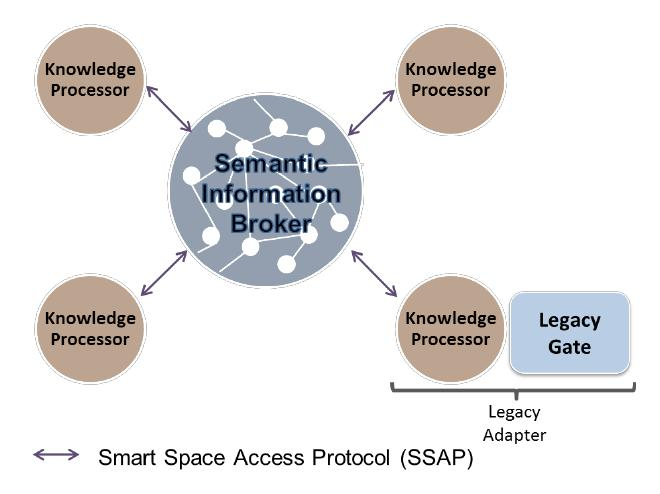
\includegraphics[width=0.5\textwidth]{assets/smart-m3.jpg}
	\caption{Architettura Smart-M3}
	\label{fig:smart-m3}
\end{figure}